% Options for packages loaded elsewhere
\PassOptionsToPackage{unicode}{hyperref}
\PassOptionsToPackage{hyphens}{url}
%
\documentclass[
]{article}
\usepackage{amsmath,amssymb}
\usepackage{lmodern}
\usepackage{iftex}
\ifPDFTeX
  \usepackage[T1]{fontenc}
  \usepackage[utf8]{inputenc}
  \usepackage{textcomp} % provide euro and other symbols
\else % if luatex or xetex
  \usepackage{unicode-math}
  \defaultfontfeatures{Scale=MatchLowercase}
  \defaultfontfeatures[\rmfamily]{Ligatures=TeX,Scale=1}
\fi
% Use upquote if available, for straight quotes in verbatim environments
\IfFileExists{upquote.sty}{\usepackage{upquote}}{}
\IfFileExists{microtype.sty}{% use microtype if available
  \usepackage[]{microtype}
  \UseMicrotypeSet[protrusion]{basicmath} % disable protrusion for tt fonts
}{}
\makeatletter
\@ifundefined{KOMAClassName}{% if non-KOMA class
  \IfFileExists{parskip.sty}{%
    \usepackage{parskip}
  }{% else
    \setlength{\parindent}{0pt}
    \setlength{\parskip}{6pt plus 2pt minus 1pt}}
}{% if KOMA class
  \KOMAoptions{parskip=half}}
\makeatother
\usepackage{xcolor}
\usepackage[margin=1in]{geometry}
\usepackage{color}
\usepackage{fancyvrb}
\newcommand{\VerbBar}{|}
\newcommand{\VERB}{\Verb[commandchars=\\\{\}]}
\DefineVerbatimEnvironment{Highlighting}{Verbatim}{commandchars=\\\{\}}
% Add ',fontsize=\small' for more characters per line
\usepackage{framed}
\definecolor{shadecolor}{RGB}{248,248,248}
\newenvironment{Shaded}{\begin{snugshade}}{\end{snugshade}}
\newcommand{\AlertTok}[1]{\textcolor[rgb]{0.94,0.16,0.16}{#1}}
\newcommand{\AnnotationTok}[1]{\textcolor[rgb]{0.56,0.35,0.01}{\textbf{\textit{#1}}}}
\newcommand{\AttributeTok}[1]{\textcolor[rgb]{0.77,0.63,0.00}{#1}}
\newcommand{\BaseNTok}[1]{\textcolor[rgb]{0.00,0.00,0.81}{#1}}
\newcommand{\BuiltInTok}[1]{#1}
\newcommand{\CharTok}[1]{\textcolor[rgb]{0.31,0.60,0.02}{#1}}
\newcommand{\CommentTok}[1]{\textcolor[rgb]{0.56,0.35,0.01}{\textit{#1}}}
\newcommand{\CommentVarTok}[1]{\textcolor[rgb]{0.56,0.35,0.01}{\textbf{\textit{#1}}}}
\newcommand{\ConstantTok}[1]{\textcolor[rgb]{0.00,0.00,0.00}{#1}}
\newcommand{\ControlFlowTok}[1]{\textcolor[rgb]{0.13,0.29,0.53}{\textbf{#1}}}
\newcommand{\DataTypeTok}[1]{\textcolor[rgb]{0.13,0.29,0.53}{#1}}
\newcommand{\DecValTok}[1]{\textcolor[rgb]{0.00,0.00,0.81}{#1}}
\newcommand{\DocumentationTok}[1]{\textcolor[rgb]{0.56,0.35,0.01}{\textbf{\textit{#1}}}}
\newcommand{\ErrorTok}[1]{\textcolor[rgb]{0.64,0.00,0.00}{\textbf{#1}}}
\newcommand{\ExtensionTok}[1]{#1}
\newcommand{\FloatTok}[1]{\textcolor[rgb]{0.00,0.00,0.81}{#1}}
\newcommand{\FunctionTok}[1]{\textcolor[rgb]{0.00,0.00,0.00}{#1}}
\newcommand{\ImportTok}[1]{#1}
\newcommand{\InformationTok}[1]{\textcolor[rgb]{0.56,0.35,0.01}{\textbf{\textit{#1}}}}
\newcommand{\KeywordTok}[1]{\textcolor[rgb]{0.13,0.29,0.53}{\textbf{#1}}}
\newcommand{\NormalTok}[1]{#1}
\newcommand{\OperatorTok}[1]{\textcolor[rgb]{0.81,0.36,0.00}{\textbf{#1}}}
\newcommand{\OtherTok}[1]{\textcolor[rgb]{0.56,0.35,0.01}{#1}}
\newcommand{\PreprocessorTok}[1]{\textcolor[rgb]{0.56,0.35,0.01}{\textit{#1}}}
\newcommand{\RegionMarkerTok}[1]{#1}
\newcommand{\SpecialCharTok}[1]{\textcolor[rgb]{0.00,0.00,0.00}{#1}}
\newcommand{\SpecialStringTok}[1]{\textcolor[rgb]{0.31,0.60,0.02}{#1}}
\newcommand{\StringTok}[1]{\textcolor[rgb]{0.31,0.60,0.02}{#1}}
\newcommand{\VariableTok}[1]{\textcolor[rgb]{0.00,0.00,0.00}{#1}}
\newcommand{\VerbatimStringTok}[1]{\textcolor[rgb]{0.31,0.60,0.02}{#1}}
\newcommand{\WarningTok}[1]{\textcolor[rgb]{0.56,0.35,0.01}{\textbf{\textit{#1}}}}
\usepackage{longtable,booktabs,array}
\usepackage{calc} % for calculating minipage widths
% Correct order of tables after \paragraph or \subparagraph
\usepackage{etoolbox}
\makeatletter
\patchcmd\longtable{\par}{\if@noskipsec\mbox{}\fi\par}{}{}
\makeatother
% Allow footnotes in longtable head/foot
\IfFileExists{footnotehyper.sty}{\usepackage{footnotehyper}}{\usepackage{footnote}}
\makesavenoteenv{longtable}
\usepackage{graphicx}
\makeatletter
\def\maxwidth{\ifdim\Gin@nat@width>\linewidth\linewidth\else\Gin@nat@width\fi}
\def\maxheight{\ifdim\Gin@nat@height>\textheight\textheight\else\Gin@nat@height\fi}
\makeatother
% Scale images if necessary, so that they will not overflow the page
% margins by default, and it is still possible to overwrite the defaults
% using explicit options in \includegraphics[width, height, ...]{}
\setkeys{Gin}{width=\maxwidth,height=\maxheight,keepaspectratio}
% Set default figure placement to htbp
\makeatletter
\def\fps@figure{htbp}
\makeatother
\setlength{\emergencystretch}{3em} % prevent overfull lines
\providecommand{\tightlist}{%
  \setlength{\itemsep}{0pt}\setlength{\parskip}{0pt}}
\setcounter{secnumdepth}{5}
\ifLuaTeX
  \usepackage{selnolig}  % disable illegal ligatures
\fi
\IfFileExists{bookmark.sty}{\usepackage{bookmark}}{\usepackage{hyperref}}
\IfFileExists{xurl.sty}{\usepackage{xurl}}{} % add URL line breaks if available
\urlstyle{same} % disable monospaced font for URLs
\hypersetup{
  pdftitle={COS-D419 Factor Analysis and Structural Equation Models 2023, Assignment 4},
  pdfauthor={Rong Guang},
  hidelinks,
  pdfcreator={LaTeX via pandoc}}

\title{COS-D419 Factor Analysis and Structural Equation Models 2023, Assignment 4}
\author{Rong Guang}
\date{2023-02-18}

\begin{document}
\maketitle

{
\setcounter{tocdepth}{2}
\tableofcontents
}
\textbf{\textcolor{blue}{The texts that reflect my understanding have been highlighted in} \textcolor{red}{red color}.}

\hypertarget{task-description}{%
\section{Task description}\label{task-description}}

The first section is task description, which is copied from the assignment5.rmd. It is for communicating with future ``me''. Please skip it.

\hypertarget{exercise-5.1}{%
\subsection{Exercise 5.1}\label{exercise-5.1}}

Specify and estimate the initial baseline models for the two groups.

Present a brief summary of the model fit and make the first step of the modification by including \textbf{(exceptionally, at the same time!)} all the four parameters known to be required for improving the model fit of both models.

Fine-tune the models step by step following the guidelines given in the lecture material, i.e., implement the modifications \textbf{(as usually, one change at a time)} testing and studying each step.

Present the final baseline models of each group and draw the graphs

\hypertarget{preparation}{%
\section{Preparation}\label{preparation}}

\#\#Read in the data set:

Start by downloading the \textbf{two data files} from Moodle to your Project folder!

\begin{Shaded}
\begin{Highlighting}[]
\CommentTok{\#install the necessary pakages}
\ControlFlowTok{if}\NormalTok{ (}\SpecialCharTok{!}\FunctionTok{require}\NormalTok{(}\StringTok{"pacman"}\NormalTok{)) }\FunctionTok{install.packages}\NormalTok{(}\StringTok{"pacman"}\NormalTok{)}
\NormalTok{pacman}\SpecialCharTok{::}\FunctionTok{p\_load}\NormalTok{(here, }
\NormalTok{               expss, }
\NormalTok{               tidyverse, }
\NormalTok{               janitor,}
\NormalTok{               knitr, }
\NormalTok{               qualtRics, }
\NormalTok{               arules, }
\NormalTok{               arulesViz, }
\NormalTok{               sjlabelled,}
\NormalTok{               DT,}
\NormalTok{               stringr,}
\NormalTok{               labelled,}
\NormalTok{               ggstatsplot,}
\NormalTok{               ggcorplot)}

\FunctionTok{library}\NormalTok{(tidyverse)}
\FunctionTok{library}\NormalTok{(readr)}

\CommentTok{\#This week\textquotesingle{}s file name}
\NormalTok{latest.name1 }\OtherTok{\textless{}{-}} \StringTok{"MBIELM1.CSV"}
\NormalTok{latest.name2 }\OtherTok{\textless{}{-}} \StringTok{"MBISEC1.CSV"}
\CommentTok{\#read in the data}
\NormalTok{mbi.elm }\OtherTok{\textless{}{-}}  \CommentTok{\#elementary school}
  \FunctionTok{read\_csv}\NormalTok{(}
    \FunctionTok{file.path}\NormalTok{(}
      \FunctionTok{here}\NormalTok{(),}
      \StringTok{\textquotesingle{}data\textquotesingle{}}\NormalTok{,}
\NormalTok{      latest.name1}
\NormalTok{      )}
\NormalTok{    )}

\NormalTok{mbi.sec }\OtherTok{\textless{}{-}} \CommentTok{\#secondary school}
  \FunctionTok{read\_csv}\NormalTok{(}
    \FunctionTok{file.path}\NormalTok{(}
      \FunctionTok{here}\NormalTok{(),}
      \StringTok{\textquotesingle{}data\textquotesingle{}}\NormalTok{,}
\NormalTok{      latest.name2}
\NormalTok{      )}
\NormalTok{    )}
\end{Highlighting}
\end{Shaded}

\hypertarget{write-functions}{%
\subsection{Write functions}\label{write-functions}}

To control length of reports, codes already shown in the previous homework were not showing in the current report. Yet they are available in .rmd report.

\hypertarget{to-generate-cfa-results-with-improved-readability}{%
\subsubsection{to generate CFA results with improved readability}\label{to-generate-cfa-results-with-improved-readability}}

\hypertarget{to-generate-a-function-for-correlation-matrix-with-numbers}{%
\subsubsection{to generate a function for correlation matrix with numbers}\label{to-generate-a-function-for-correlation-matrix-with-numbers}}

\hypertarget{to-generate-a-function-for-histogram-overlapping-with-density-plot}{%
\subsubsection{to generate a function for histogram overlapping with density plot}\label{to-generate-a-function-for-histogram-overlapping-with-density-plot}}

\hypertarget{to-generate-a-function-for-violin-overlapping-with-box-plot}{%
\subsubsection{to generate a function for violin overlapping with box plot}\label{to-generate-a-function-for-violin-overlapping-with-box-plot}}

\hypertarget{to-generate-a-function-describing-continuous-data-set}{%
\subsubsection{To generate a function describing continuous data set}\label{to-generate-a-function-describing-continuous-data-set}}

\hypertarget{write-a-function-describing-continuous-data-set}{%
\subsubsection{Write a function describing continuous data set}\label{write-a-function-describing-continuous-data-set}}

\hypertarget{write-a-function-for-histogram-overlapping-with-density-plot}{%
\subsubsection{Write a function for histogram overlapping with density plot}\label{write-a-function-for-histogram-overlapping-with-density-plot}}

\hypertarget{write-a-function-to-generate-dot-distribution-plot}{%
\subsubsection{Write a function to generate dot distribution plot}\label{write-a-function-to-generate-dot-distribution-plot}}

\begin{Shaded}
\begin{Highlighting}[]
\NormalTok{dot.dist }\OtherTok{\textless{}{-}} 
  \ControlFlowTok{function}\NormalTok{(data, type, title)\{}
\NormalTok{    data }\SpecialCharTok{|\textgreater{}}
      \FunctionTok{t}\NormalTok{() }\SpecialCharTok{|\textgreater{}} 
      \FunctionTok{as.data.frame}\NormalTok{() }\SpecialCharTok{\%\textgreater{}\%} 
      \FunctionTok{mutate}\NormalTok{(}\AttributeTok{Item =} \FunctionTok{rownames}\NormalTok{(.)) }\SpecialCharTok{|\textgreater{}} 
      \FunctionTok{rowwise}\NormalTok{() }\SpecialCharTok{|\textgreater{}} 
      \FunctionTok{mutate}\NormalTok{(}\AttributeTok{Median =} \FunctionTok{eval}\NormalTok{(}\FunctionTok{parse}\NormalTok{(}\AttributeTok{text =}\NormalTok{ type))(V1}\SpecialCharTok{:}\NormalTok{V580)) }\SpecialCharTok{|\textgreater{}} 
\NormalTok{      ggstatsplot}\SpecialCharTok{::}\FunctionTok{ggdotplotstats}\NormalTok{(}
        \AttributeTok{point.args =} \FunctionTok{list}\NormalTok{(}\AttributeTok{color =} \StringTok{"red"}\NormalTok{, }\AttributeTok{size =} \DecValTok{3}\NormalTok{, }\AttributeTok{shape =} \DecValTok{13}\NormalTok{),}
        \AttributeTok{xlab =} \FunctionTok{paste}\NormalTok{(type, }\StringTok{"ratings"}\NormalTok{),}
        \AttributeTok{title =}\NormalTok{ title,}
        \AttributeTok{x =}\NormalTok{ Median,}
        \AttributeTok{y =}\NormalTok{ Item}
\NormalTok{      )}
\NormalTok{    \}}
\end{Highlighting}
\end{Shaded}

\hypertarget{write-a-fuction-to-generate-correlation-matrix-with-statistical-test}{%
\subsubsection{Write a fuction to generate correlation matrix with statistical test}\label{write-a-fuction-to-generate-correlation-matrix-with-statistical-test}}

\begin{Shaded}
\begin{Highlighting}[]
\NormalTok{mycor }\OtherTok{\textless{}{-}} 
  \ControlFlowTok{function}\NormalTok{(data, cols, title)\{}
\NormalTok{  mbi.elm }\SpecialCharTok{|\textgreater{}} 
      \FunctionTok{select}\NormalTok{(}\FunctionTok{all\_of}\NormalTok{(cols)) }\SpecialCharTok{|\textgreater{}} 
\NormalTok{      ggstatsplot}\SpecialCharTok{::}\FunctionTok{ggcorrmat}\NormalTok{(}
        \AttributeTok{colors =} \FunctionTok{c}\NormalTok{(}\StringTok{"\#B2182B"}\NormalTok{, }\StringTok{"white"}\NormalTok{, }\StringTok{"\#4D4D4D"}\NormalTok{),}
        \AttributeTok{title =} \StringTok{"(a) Items on emotional exhaustion, }
\StringTok{        elementary school teacher"}\NormalTok{,}
        \AttributeTok{matrix.type  =} \StringTok{"lower"}
\NormalTok{      )}
\NormalTok{    \}}
\end{Highlighting}
\end{Shaded}

\hypertarget{inspect-the-data}{%
\section{Inspect the data}\label{inspect-the-data}}

\hypertarget{distribution}{%
\subsection{Distribution}\label{distribution}}

\begin{Shaded}
\begin{Highlighting}[]
\CommentTok{\#generate the plots, by subgroup of teachers}
\NormalTok{p.dist.elm }\OtherTok{\textless{}{-}} 
  \FunctionTok{corr.density}\NormalTok{(}
\NormalTok{    mbi.elm, }
    \AttributeTok{fig.num =} \StringTok{"1(a)"}\NormalTok{, }
    \AttributeTok{group =} \StringTok{"elementary school teacher"}
\NormalTok{    )}
\NormalTok{p.dist.sec }\OtherTok{\textless{}{-}} 
  \FunctionTok{corr.density}\NormalTok{(}
\NormalTok{    mbi.sec, }
    \AttributeTok{fig.num =} \StringTok{"1(b)"}\NormalTok{,}
    \AttributeTok{group =} \StringTok{"secondary school teacher"}
\NormalTok{    )}
\CommentTok{\#print the plot}
\FunctionTok{library}\NormalTok{(patchwork); p.dist.elm}\SpecialCharTok{/}\NormalTok{p.dist.sec}
\end{Highlighting}
\end{Shaded}

\begin{center}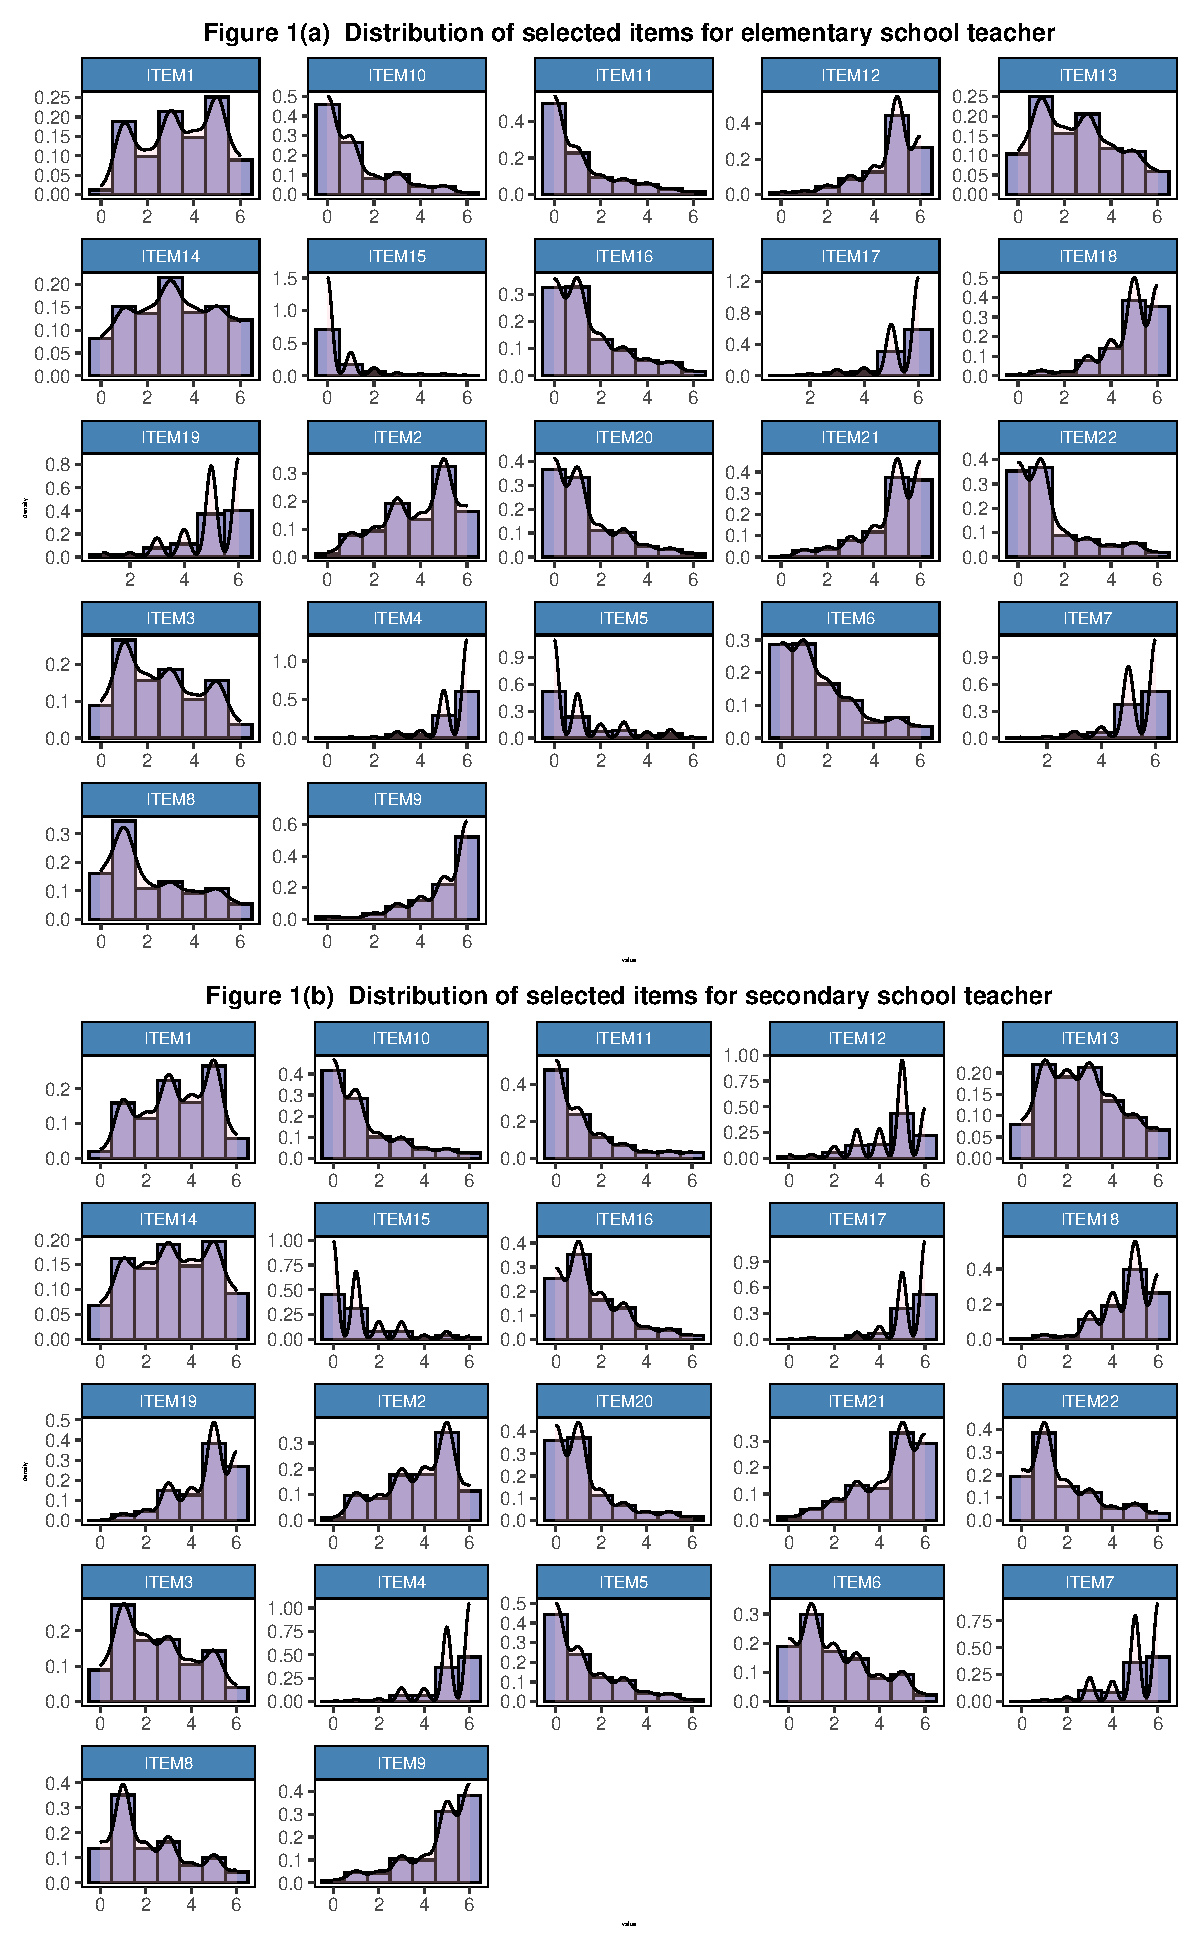
\includegraphics{Assignment5_RongGuang_files/figure-latex/unnamed-chunk-11-1} \end{center}

\begin{Shaded}
\begin{Highlighting}[]
\CommentTok{\#generate plot by subgroups of teachers}
\NormalTok{p.dot.elm }\OtherTok{\textless{}{-}} 
  \FunctionTok{dot.dist}\NormalTok{(}
    \AttributeTok{data =}\NormalTok{ mbi.elm, }
    \AttributeTok{type =} \StringTok{"median"}\NormalTok{, }
    \AttributeTok{title =} \StringTok{"(a) Elementary school teacher"}
\NormalTok{    )}
\NormalTok{p.dot.sec }\OtherTok{\textless{}{-}} 
  \FunctionTok{dot.dist}\NormalTok{(}
    \AttributeTok{data =}\NormalTok{ mbi.sec, }
    \AttributeTok{type =} \StringTok{"median"}\NormalTok{, }
    \AttributeTok{title =} \StringTok{"(b) Secondary school teacher"}
\NormalTok{    )}
\CommentTok{\#plot layout}
\NormalTok{patchwork }\OtherTok{\textless{}{-}}\NormalTok{ p.dot.elm}\SpecialCharTok{|}\NormalTok{p.dot.sec}
\CommentTok{\#print the plot with a genral title}
\NormalTok{patchwork}\SpecialCharTok{+}\FunctionTok{plot\_annotation}\NormalTok{(}
    \AttributeTok{title =} 
      \StringTok{\textquotesingle{}Figure 2 Distributions of median rating for each item\textquotesingle{}}\NormalTok{,}
    \AttributeTok{theme =} 
      \FunctionTok{theme}\NormalTok{(}\AttributeTok{plot.title =} 
              \FunctionTok{element\_text}\NormalTok{(}
                \AttributeTok{size =} \DecValTok{16}\NormalTok{,}
                \AttributeTok{face =} \StringTok{"bold"}\NormalTok{,}
                \AttributeTok{vjust =} \SpecialCharTok{{-}}\FloatTok{1.5}\NormalTok{,}
                \AttributeTok{hjust =}\FloatTok{0.5}\NormalTok{)}
\NormalTok{            )}
\NormalTok{    )}
\end{Highlighting}
\end{Shaded}

\begin{center}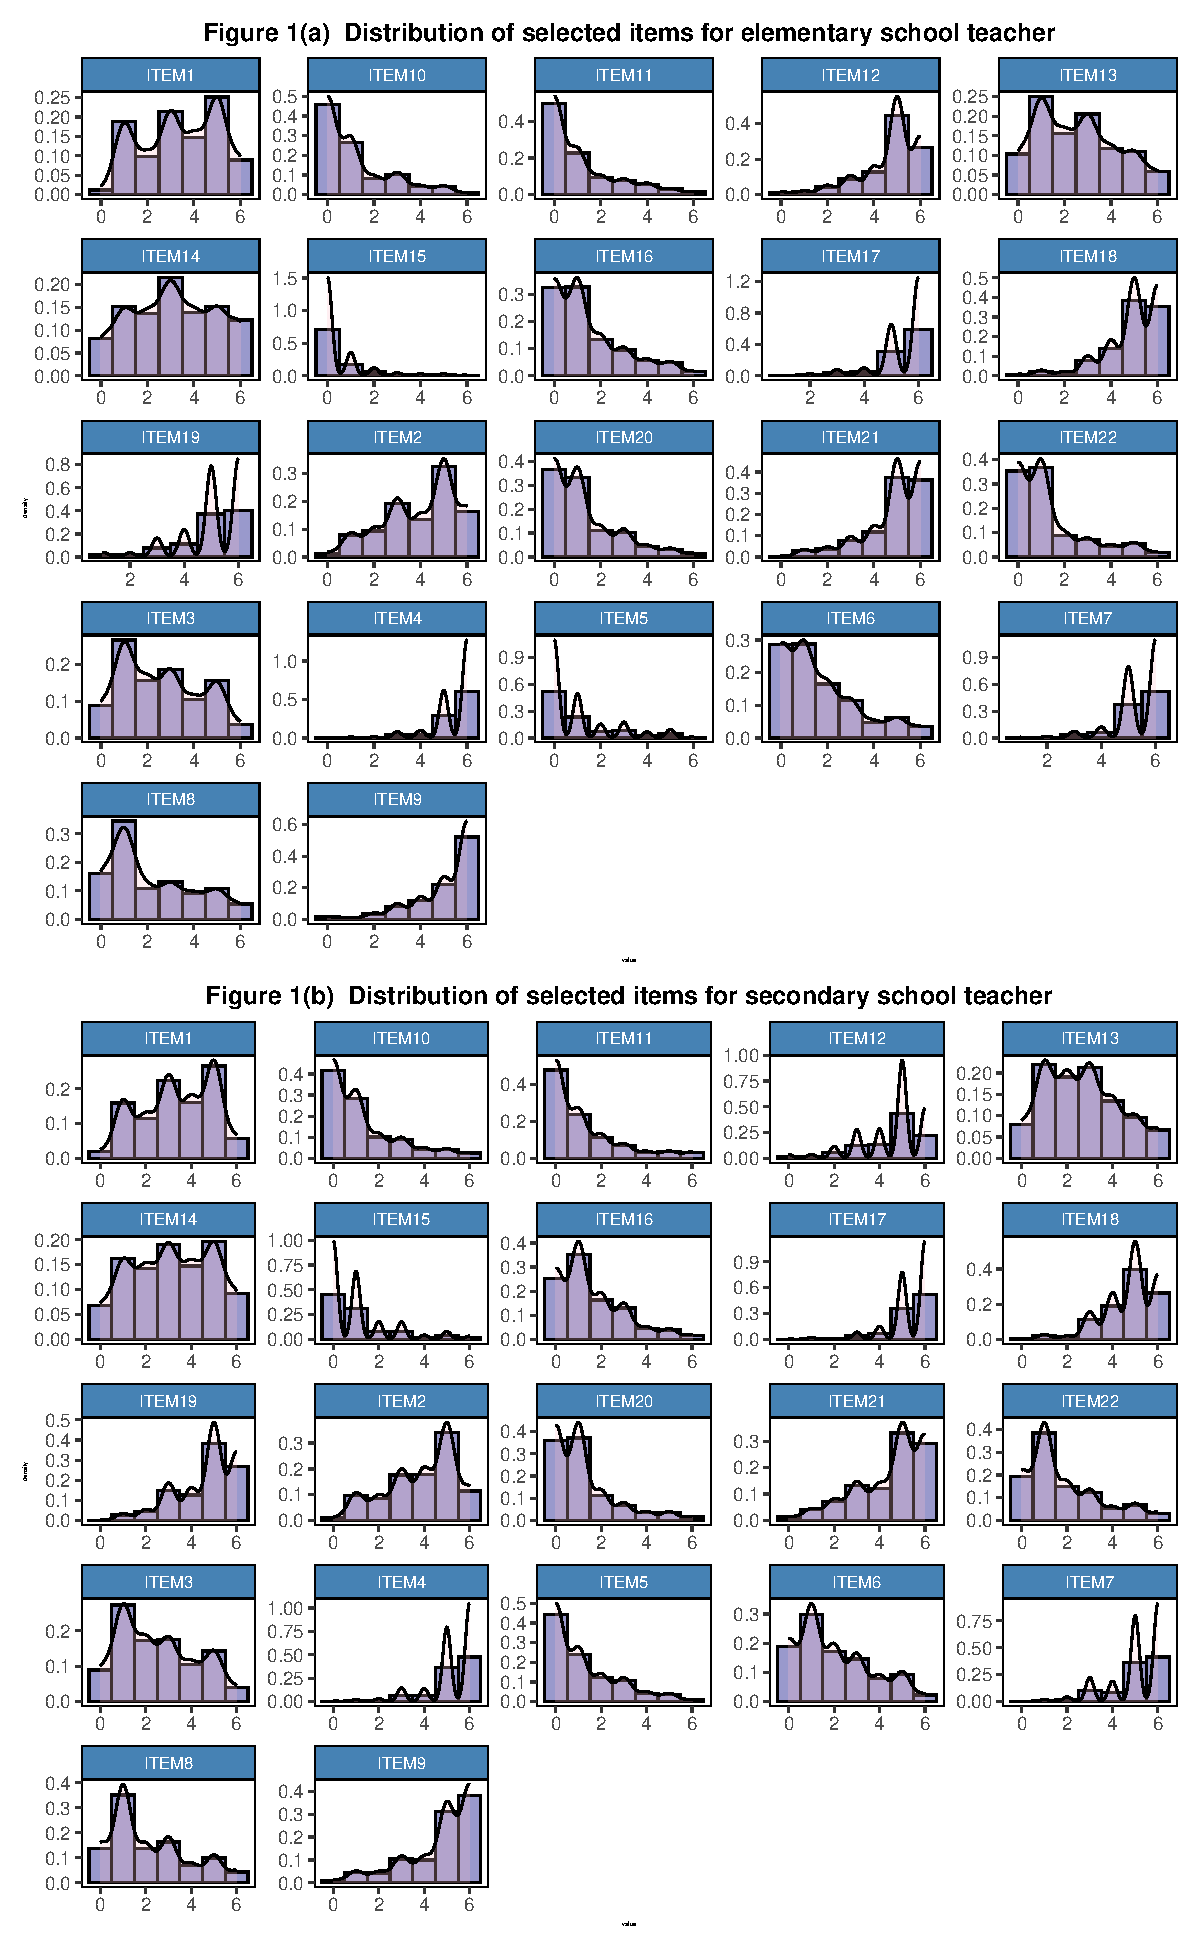
\includegraphics{Assignment5_RongGuang_files/figure-latex/unnamed-chunk-12-1} \end{center}

\begin{Shaded}
\begin{Highlighting}[]
\NormalTok{fa.ee }\OtherTok{\textless{}{-}} \FunctionTok{c}\NormalTok{(}\StringTok{"ITEM1"}\NormalTok{, }\StringTok{"ITEM3"}\NormalTok{, }\StringTok{"ITEM6"}\NormalTok{, }\StringTok{"ITEM8"}\NormalTok{, }\StringTok{"ITEM13"}\NormalTok{, }\StringTok{"ITEM14"}\NormalTok{, }\StringTok{"ITEM16"}\NormalTok{, }\StringTok{"ITEM20"}\NormalTok{)}
\NormalTok{fa.dp }\OtherTok{\textless{}{-}} \FunctionTok{c}\NormalTok{(}\StringTok{"ITEM5"}\NormalTok{, }\StringTok{"ITEM10"}\NormalTok{, }\StringTok{"ITEM11"}\NormalTok{, }\StringTok{"ITEM15"}\NormalTok{, }\StringTok{"ITEM22"}\NormalTok{)}
\NormalTok{fa.pa }\OtherTok{\textless{}{-}} \FunctionTok{c}\NormalTok{(}\StringTok{"ITEM4"}\NormalTok{, }\StringTok{"ITEM7"}\NormalTok{, }\StringTok{"ITEM9"}\NormalTok{, }\StringTok{"ITEM12"}\NormalTok{, }\StringTok{"ITEM17"}\NormalTok{, }\StringTok{"ITEM18"}\NormalTok{, }\StringTok{"ITEM19"}\NormalTok{, }\StringTok{"ITEM21"}\NormalTok{)}
\CommentTok{\#generate 6 plots, 3 factors X 2 subgroups of teachers}
\NormalTok{p.cor.elm.ee }\OtherTok{\textless{}{-}} 
       \FunctionTok{mycor}\NormalTok{(}
         \AttributeTok{data=}\NormalTok{ mbi.elm, }
         \AttributeTok{cols =}\NormalTok{ fa.ee, }
         \StringTok{"(a) Items on emotional exhaustion, }
\StringTok{         elementary school teacher"}
\NormalTok{         )}
\NormalTok{p.cor.sec.ee }\OtherTok{\textless{}{-}} 
       \FunctionTok{mycor}\NormalTok{(}
         \AttributeTok{data =}\NormalTok{ mbi.sec, }
         \AttributeTok{cols =}\NormalTok{ fa.ee, }
         \StringTok{"(b) Items on emotional exhaustion, }
\StringTok{          secondary school teacher"}
\NormalTok{         )}
\NormalTok{p.cor.elm.dp }\OtherTok{\textless{}{-}} 
       \FunctionTok{mycor}\NormalTok{(}
         \AttributeTok{data =}\NormalTok{ mbi.elm, }
         \AttributeTok{cols =}\NormalTok{ fa.dp, }
         \StringTok{"(c) Items on depersonalization,}
\StringTok{          elementary school teacher"}
\NormalTok{         )}
\NormalTok{p.cor.sec.dp }\OtherTok{\textless{}{-}} 
       \FunctionTok{mycor}\NormalTok{(}
         \AttributeTok{data =}\NormalTok{ mbi.sec, }
         \AttributeTok{cols =}\NormalTok{ fa.dp, }
         \StringTok{"(d) Items on depersonalization,}
\StringTok{          secondary school teacher"}
\NormalTok{         )}
\NormalTok{p.cor.elm.pa }\OtherTok{\textless{}{-}} 
       \FunctionTok{mycor}\NormalTok{(}
         \AttributeTok{data =}\NormalTok{ mbi.elm, }
         \AttributeTok{cols =}\NormalTok{ fa.pa, }
         \StringTok{"(e) Items on personal accomplishment,}
\StringTok{         secondary school teacher"}
\NormalTok{         )}
\NormalTok{p.cor.sec.pa }\OtherTok{\textless{}{-}} 
       \FunctionTok{mycor}\NormalTok{(}
         \AttributeTok{data =}\NormalTok{ mbi.sec ,}
         \AttributeTok{cols =}\NormalTok{ fa.pa, }
         \StringTok{"(f) Items on personal accomplishment,}
\StringTok{          secondary school teacher"}
\NormalTok{         )}
\CommentTok{\#plot sub{-}figure layout}
\NormalTok{patchwork }\OtherTok{\textless{}{-}} 
\NormalTok{  p.cor.elm.ee}\SpecialCharTok{/}\NormalTok{p.cor.elm.dp}\SpecialCharTok{/}\NormalTok{p.cor.elm.pa}\SpecialCharTok{|}\NormalTok{p.cor.sec.ee}\SpecialCharTok{/}\NormalTok{p.cor.sec.dp}\SpecialCharTok{/}\NormalTok{p.cor.sec.pa }
\CommentTok{\#print the plot with a gernal title}
\NormalTok{patchwork}\SpecialCharTok{+}
  \FunctionTok{plot\_annotation}\NormalTok{(}
    \AttributeTok{title =} 
      \StringTok{\textquotesingle{}Figure 3 Correlalogram for items on each factor for two groups of teachers\textquotesingle{}}\NormalTok{,}
    \AttributeTok{theme =} 
      \FunctionTok{theme}\NormalTok{(}\AttributeTok{plot.title =} 
              \FunctionTok{element\_text}\NormalTok{(}
                \AttributeTok{size =} \DecValTok{16}\NormalTok{,}
                \AttributeTok{face =} \StringTok{"bold"}\NormalTok{,}
                \AttributeTok{vjust =} \SpecialCharTok{{-}}\FloatTok{1.5}\NormalTok{,}
                \AttributeTok{hjust =}\FloatTok{0.5}\NormalTok{)}
\NormalTok{            )}
\NormalTok{    )}
\end{Highlighting}
\end{Shaded}

\begin{center}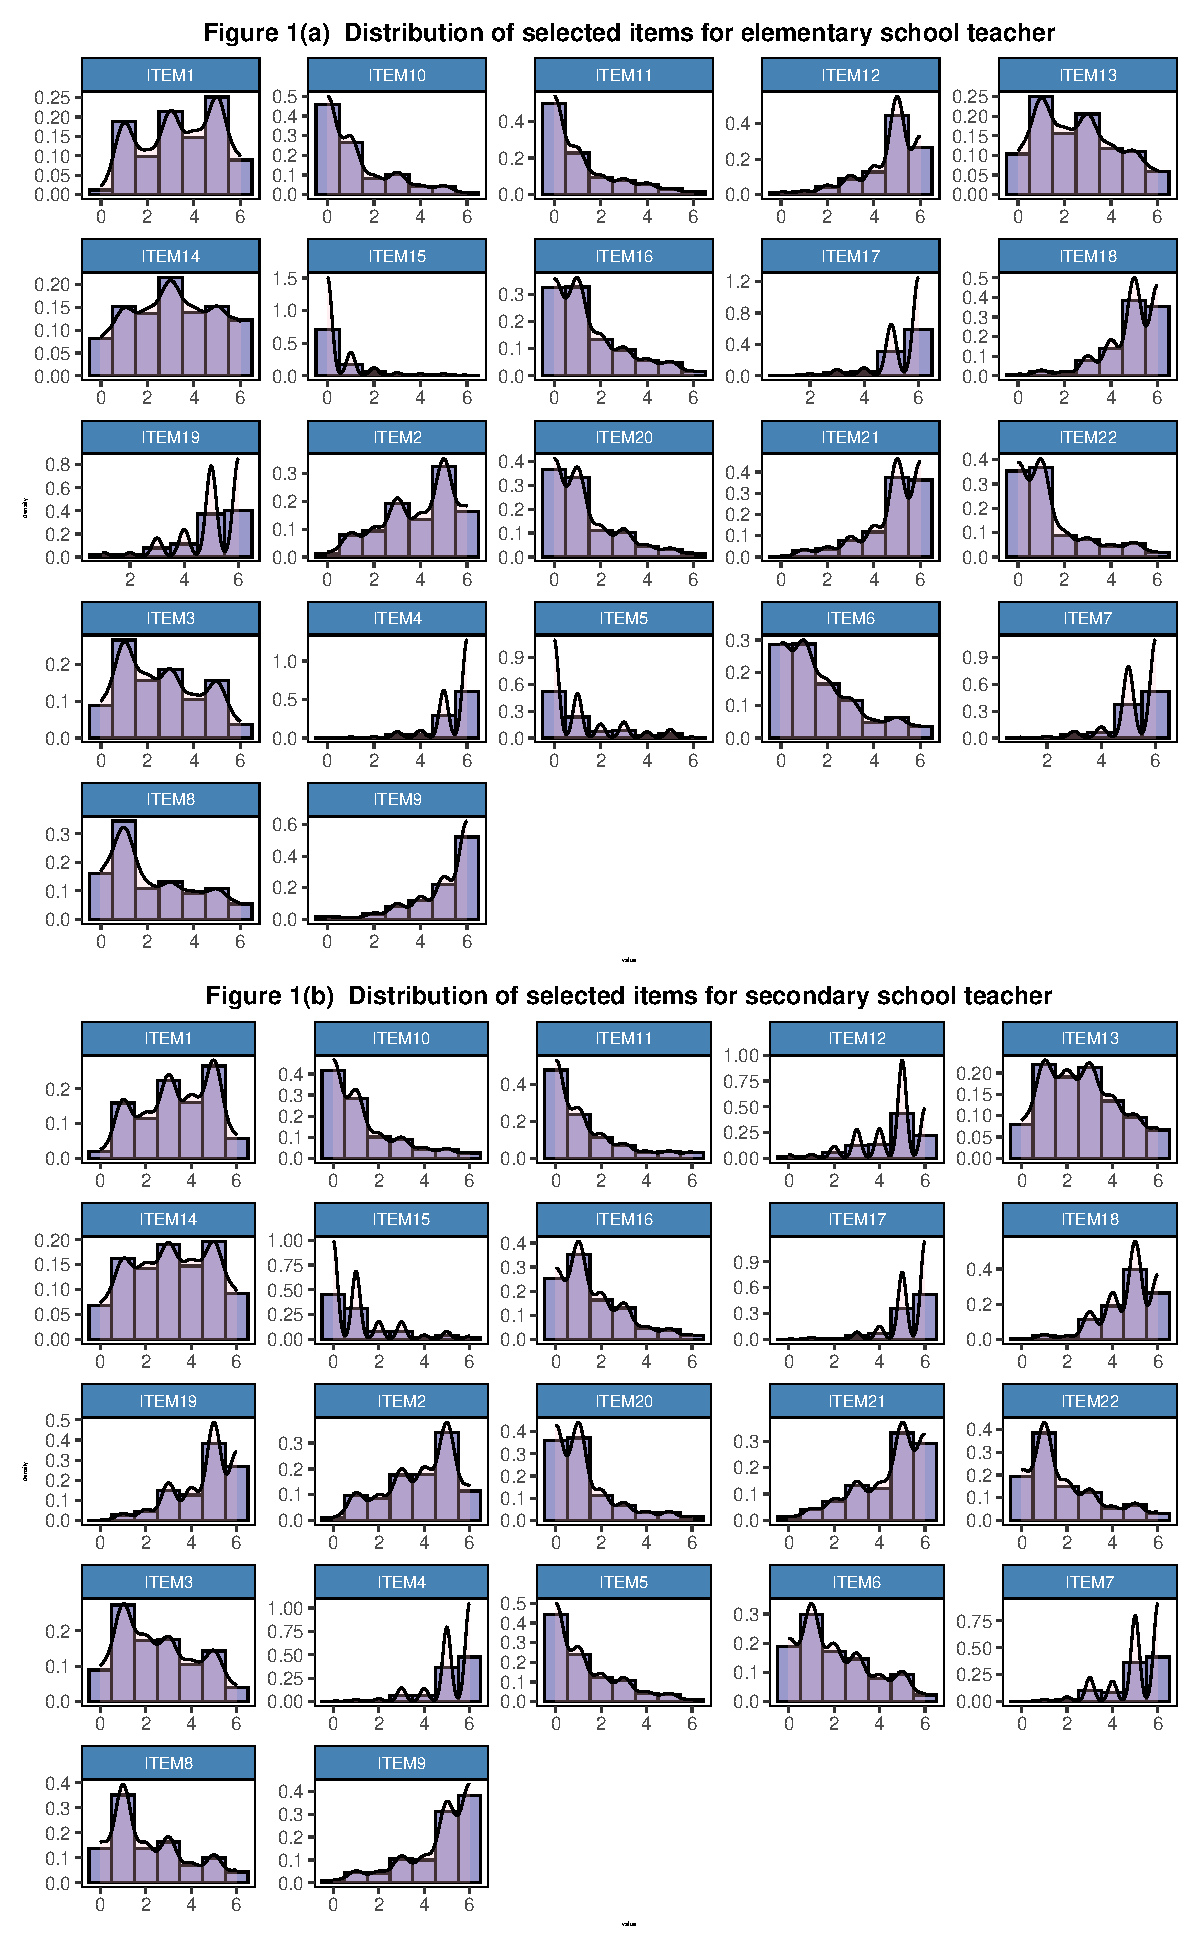
\includegraphics{Assignment5_RongGuang_files/figure-latex/unnamed-chunk-13-1} \end{center}

\hypertarget{testing-the-factorial-invariance-of-mbi-inventory-between-elementary-and-secondary-school-teachers}{%
\section{Testing the factorial invariance of MBI inventory between elementary and secondary school teachers}\label{testing-the-factorial-invariance-of-mbi-inventory-between-elementary-and-secondary-school-teachers}}

\hypertarget{define-and-estimate-initial-models-for-both-subgroups}{%
\subsection{Define and estimate initial models for both subgroups}\label{define-and-estimate-initial-models-for-both-subgroups}}

The model under test in this initial multi-group application is the same postulated three-factor structure of the MBI that was tested in the previous assignments.

\hypertarget{define-the-baseline-model}{%
\subsubsection{Define the baseline model}\label{define-the-baseline-model}}

\begin{Shaded}
\begin{Highlighting}[]
\FunctionTok{library}\NormalTok{(lavaan)}
\CommentTok{\# Define a CFA model using the lavaan (Latent Variable Analysis) syntax:}
\CommentTok{\# see https://lavaan.ugent.be/tutorial/syntax1.html}
\NormalTok{BLmodel }\OtherTok{\textless{}{-}} \StringTok{\textquotesingle{}}
\StringTok{\# CFA model for the burnout, the baseline model:}
\StringTok{    EE =\textasciitilde{} ITEM1 + ITEM2 + ITEM3 + ITEM6 + ITEM8 + }
\StringTok{          ITEM13 + ITEM14 + ITEM16 + ITEM20}
\StringTok{    DP =\textasciitilde{} ITEM5 + ITEM10 + ITEM11 + ITEM15 +ITEM22}
\StringTok{    PA =\textasciitilde{} ITEM4 + ITEM7 + ITEM9 + ITEM12 + }
\StringTok{          ITEM17 + ITEM18 + ITEM19 + ITEM21}
\StringTok{          \textquotesingle{}}
\end{Highlighting}
\end{Shaded}

It is important to note that measuring instruments are often group specific in the way they operate, and, thus, it is possible that baseline models may not be completely identical across groups

\hypertarget{estimate-factorial-validity}{%
\subsubsection{Estimate factorial validity}\label{estimate-factorial-validity}}

\begin{enumerate}
\def\labelenumi{(\arabic{enumi})}
\tightlist
\item
  Estimate factorial validity for the elementary teacher subgroup
\end{enumerate}

\begin{Shaded}
\begin{Highlighting}[]
\NormalTok{cfa.elm }\OtherTok{\textless{}{-}} 
  \FunctionTok{cfa}\NormalTok{(}
\NormalTok{    BLmodel, }
    \AttributeTok{data =}\NormalTok{ mbi.elm,  }
    \AttributeTok{estimator =} \StringTok{"MLM"}\NormalTok{,}
    \AttributeTok{mimic =} \StringTok{"Mplus"}
\NormalTok{    )}
\end{Highlighting}
\end{Shaded}

\begin{enumerate}
\def\labelenumi{(\arabic{enumi})}
\setcounter{enumi}{1}
\tightlist
\item
  Estimate factorial validity for the secondary teacher subgroup
\end{enumerate}

\begin{Shaded}
\begin{Highlighting}[]
\NormalTok{cfa.sec }\OtherTok{\textless{}{-}} 
  \FunctionTok{cfa}\NormalTok{(}
\NormalTok{    BLmodel, }
    \AttributeTok{data =}\NormalTok{ mbi.sec,  }
    \AttributeTok{estimator =} \StringTok{"MLM"}\NormalTok{,}
    \AttributeTok{mimic =} \StringTok{"Mplus"}
\NormalTok{    )}
\end{Highlighting}
\end{Shaded}

\hypertarget{evaluate-model-fit}{%
\subsubsection{Evaluate model fit}\label{evaluate-model-fit}}

\begin{Shaded}
\begin{Highlighting}[]
\FunctionTok{library}\NormalTok{(knitr);}\FunctionTok{library}\NormalTok{(kableExtra)}
\NormalTok{BL.elm.fit }\OtherTok{\textless{}{-}} \FunctionTok{cfa.summary.mlm.a}\NormalTok{(cfa.elm) }\SpecialCharTok{|\textgreater{}} \FunctionTok{t}\NormalTok{() }\SpecialCharTok{|\textgreater{}} \FunctionTok{as.data.frame}\NormalTok{()}
\NormalTok{BL.sec.fit }\OtherTok{\textless{}{-}} \FunctionTok{cfa.summary.mlm.a}\NormalTok{(cfa.sec) }\SpecialCharTok{|\textgreater{}} \FunctionTok{t}\NormalTok{() }\SpecialCharTok{|\textgreater{}} \FunctionTok{as.data.frame}\NormalTok{()}
\NormalTok{BL.both }\OtherTok{\textless{}{-}} \FunctionTok{rbind}\NormalTok{(BL.elm.fit[}\DecValTok{2}\NormalTok{,], BL.sec.fit[}\DecValTok{2}\NormalTok{,]) }
\FunctionTok{names}\NormalTok{(BL.both) }\OtherTok{\textless{}{-}}\NormalTok{ BL.elm.fit[}\DecValTok{1}\NormalTok{,]}
\FunctionTok{rownames}\NormalTok{(BL.both) }\OtherTok{\textless{}{-}} \FunctionTok{c}\NormalTok{(}\StringTok{"Elementary School Teachers"}\NormalTok{,}
                       \StringTok{"Secondary School Tearchers"}\NormalTok{)}

\NormalTok{BL.both }\OtherTok{\textless{}{-}}\NormalTok{ BL.both }\SpecialCharTok{|\textgreater{}} 
  \FunctionTok{rename}\NormalTok{(}\AttributeTok{p =} \StringTok{\textquotesingle{}p value\textquotesingle{}}\NormalTok{,}
         \AttributeTok{p2 =} \StringTok{\textquotesingle{}RMSEA p value\textquotesingle{}}\NormalTok{,}
         \AttributeTok{chi =} \StringTok{\textquotesingle{}chi square\textquotesingle{}}\NormalTok{) }\SpecialCharTok{|\textgreater{}} 
  \FunctionTok{mutate}\NormalTok{(}\AttributeTok{df =} \FunctionTok{as.numeric}\NormalTok{(df) }\SpecialCharTok{|\textgreater{}} \FunctionTok{round}\NormalTok{(}\DecValTok{0}\NormalTok{),}
         \AttributeTok{p =} \FunctionTok{case\_when}\NormalTok{(}
           \FunctionTok{as.numeric}\NormalTok{(p) }\SpecialCharTok{\textless{}} \FloatTok{0.001} \SpecialCharTok{\textasciitilde{}} \StringTok{"\textless{}0.001"}\NormalTok{,}
           \FunctionTok{as.numeric}\NormalTok{(p) }\SpecialCharTok{\textgreater{}=} \FloatTok{0.001} \SpecialCharTok{\textasciitilde{}}\NormalTok{ p}
\NormalTok{           ),}
         \AttributeTok{p2 =} \FunctionTok{case\_when}\NormalTok{(}
           \FunctionTok{as.numeric}\NormalTok{(p2) }\SpecialCharTok{\textless{}} \FloatTok{0.001} \SpecialCharTok{\textasciitilde{}} \StringTok{"\textless{}0.001"}\NormalTok{,}
           \FunctionTok{as.numeric}\NormalTok{(p2) }\SpecialCharTok{\textgreater{}=} \FloatTok{0.001} \SpecialCharTok{\textasciitilde{}}\NormalTok{ p2}
\NormalTok{           )}
\NormalTok{         ) }\SpecialCharTok{|\textgreater{}}
  \FunctionTok{mutate}\NormalTok{(}\StringTok{\textquotesingle{}Chi square (df, p)\textquotesingle{}} \OtherTok{=} 
           \FunctionTok{paste0}\NormalTok{(chi, }\StringTok{"("}\NormalTok{, df,}\StringTok{", "}\NormalTok{, p, }\StringTok{")"}\NormalTok{),}
         \StringTok{\textquotesingle{}RMSEA(p)\textquotesingle{}}           \OtherTok{=} 
           \FunctionTok{paste0}\NormalTok{(RMSEA, }\StringTok{"("}\NormalTok{, p2, }\StringTok{")"}
\NormalTok{                  )}
\NormalTok{         ) }\SpecialCharTok{|\textgreater{}} 
  \FunctionTok{select}\NormalTok{(}\StringTok{\textquotesingle{}Chi square (df, p)\textquotesingle{}}\NormalTok{, }
\NormalTok{         CFI, TLI, }
         \StringTok{\textquotesingle{}RMSEA(p)\textquotesingle{}}\NormalTok{, }
\NormalTok{         SRMR, }
         \StringTok{\textquotesingle{}CSF*\textquotesingle{}}\OtherTok{=}\NormalTok{ CSF}
\NormalTok{         ) }

\NormalTok{BL.both }\SpecialCharTok{|\textgreater{}} 
  \FunctionTok{kable}\NormalTok{(}\AttributeTok{booktabs =}\NormalTok{ T, }
        \CommentTok{\#format = "markdown", }
        \AttributeTok{caption =} 
          \StringTok{"Fit indices for two subgroups, basline models"}\NormalTok{,}
        \AttributeTok{align =} \StringTok{"r"}
\NormalTok{        ) }\SpecialCharTok{|\textgreater{}} 
  \FunctionTok{kable\_styling}\NormalTok{(}\AttributeTok{full\_width =}\NormalTok{ T) }\SpecialCharTok{|\textgreater{}} 
  \FunctionTok{footnote}\NormalTok{(}\AttributeTok{symbol =} 
             \StringTok{"Chi square scaling factor"}
\NormalTok{           ) }\SpecialCharTok{|\textgreater{}}
  \FunctionTok{column\_spec}\NormalTok{(}\DecValTok{1}\NormalTok{, }\AttributeTok{width =} \StringTok{"3.5cm"}\NormalTok{) }\SpecialCharTok{|\textgreater{}} 
  \FunctionTok{column\_spec}\NormalTok{(}\DecValTok{2}\NormalTok{, }\AttributeTok{width =} \StringTok{"4cm"}\NormalTok{)}\SpecialCharTok{|\textgreater{}} 
  \FunctionTok{column\_spec}\NormalTok{(}\DecValTok{3}\NormalTok{, }\AttributeTok{width =} \StringTok{"1cm"}\NormalTok{)}\SpecialCharTok{|\textgreater{}} 
  \FunctionTok{column\_spec}\NormalTok{(}\DecValTok{4}\NormalTok{, }\AttributeTok{width =} \StringTok{"1cm"}\NormalTok{)}\SpecialCharTok{|\textgreater{}} 
  \FunctionTok{column\_spec}\NormalTok{(}\DecValTok{5}\NormalTok{, }\AttributeTok{width =} \StringTok{"2.5cm"}\NormalTok{)}\SpecialCharTok{|\textgreater{}} 
  \FunctionTok{column\_spec}\NormalTok{(}\DecValTok{6}\NormalTok{, }\AttributeTok{width =} \StringTok{"1cm"}\NormalTok{) }\SpecialCharTok{|\textgreater{}} 
  \FunctionTok{column\_spec}\NormalTok{(}\DecValTok{7}\NormalTok{, }\AttributeTok{width =} \StringTok{"1cm"}\NormalTok{) }
\end{Highlighting}
\end{Shaded}

\begin{table}

\caption{\label{tab:unnamed-chunk-17}Fit indices for two subgroups, basline models}
\centering
\begin{tabu} to \linewidth {>{\raggedright\arraybackslash}p{3.5cm}>{\raggedleft\arraybackslash}p{4cm}>{\raggedleft\arraybackslash}p{1cm}>{\raggedleft\arraybackslash}p{1cm}>{\raggedleft\arraybackslash}p{2.5cm}>{\raggedleft\arraybackslash}p{1cm}>{\raggedleft\arraybackslash}p{1cm}}
\toprule
  & Chi square (df, p) & CFI & TLI & RMSEA(p) & SRMR & CSF*\\
\midrule
Elementary School Teachers & 826.573(206, <0.001) & 0.857 & 0.840 & 0.072(<0.001) & 0.068 & 1.225\\
Secondary School Tearchers & 999.359(206, <0.001) & 0.836 & 0.816 & 0.075(<0.001) & 0.077 & 1.284\\
\bottomrule
\multicolumn{7}{l}{\rule{0pt}{1em}\textsuperscript{*} Chi square scaling factor}\\
\end{tabu}
\end{table}

\textcolor{blue}{See table 1. Goodness-of-fit statistics for this baseline model (three factor) reveals that the indices are less than optimal for both elementary (MLM Chi-square[206] = 826.573; CFI = 0.857; RMSEA = 0.072 ; SRMR = 0.068) and secondary (MLM Chi-square[206] = 999.359; CFI = 0.836; RMSEA = 0.075; SRMR = 0.077) levels.}

\textcolor{blue}{The texts that reflect my understanding have been highlighted in}

\end{document}
